\documentclass[11pt]{article}
\usepackage{../latex/colombiamacro}
\usepackage{needspace}
\graphicspath{{../figuras/}{../img/}{../presentacion/}}
\setlength{\emergencystretch}{2.5em}
\fancyhead[L]{\sffamily\footnotesize\color{cmmuted}ColombiaMacro · Guía de presentación académica}

% Ficha de un grafico. \grafico: imagen a la izquierda y texto a la derecha; \graficoancho: imagen arriba.
\newcommand{\lab}[1]{\raggedright{\sffamily\bfseries\footnotesize\color{cmblue}\MakeUppercase{#1}}\\[1pt]}
\newcommand{\fichatexto}[3]{\lab{Construcción}#1\par\smallskip\lab{Lectura}#2\par\smallskip\lab{Para el inversionista}#3}
\newcommand{\grafico}[5]{\par\noindent
\begin{minipage}[c]{0.44\linewidth}\includegraphics[width=\linewidth]{#1}\end{minipage}\hfill
\begin{minipage}[c]{0.53\linewidth}\small\setlength{\parskip}{0pt}\fichatexto{#3}{#4}{#5}\end{minipage}\par\bigskip}
\newcommand{\graficoancho}[5]{\par\noindent
\begin{minipage}{\linewidth}\centering\includegraphics[width=#2\linewidth]{#1}\par\medskip
\raggedright\small\setlength{\parskip}{0pt}
\begin{minipage}[t]{0.32\linewidth}\lab{Construcción}#3\end{minipage}\hfill
\begin{minipage}[t]{0.32\linewidth}\lab{Lectura}#4\end{minipage}\hfill
\begin{minipage}[t]{0.32\linewidth}\lab{Para el inversionista}#5\end{minipage}\end{minipage}\par\bigskip}
\newcommand{\di}[1]{\textit{“#1”}}

\begin{document}

% ================================================================
\begin{titlepage}
\thispagestyle{empty}
\begin{tikzpicture}[remember picture,overlay]
  \fill[cmink] (current page.north west) rectangle ([yshift=-9mm]current page.north east);
\end{tikzpicture}
\vspace*{16mm}
{\sffamily\small\color{cmmuted}UNIVERSIDAD DE SAN BUENAVENTURA CALI · FINANZAS Y NEGOCIOS INTERNACIONALES\par}
\vspace{14mm}
{\sffamily\bfseries\fontsize{32}{38}\selectfont ColombiaMacro\\[2mm]\fontsize{20}{26}\selectfont Guía para la presentación académica\par}
\vspace{6mm}
{\large Datos, construcción de los gráficos, interpretación y lectura para inversionistas\par}
\vspace{10mm}
\begin{tcolorbox}[colback=cmsoft,colframe=cmsoft,arc=2pt,left=10pt,right=10pt,top=8pt,bottom=8pt]
\sffamily\textbf{Pregunta de la presentación}\\[3pt]
\normalfont ¿En qué fase del ciclo está la economía colombiana y qué implica para la inflación, la política
monetaria y los precios de los activos?\\[6pt]
\sffamily\textbf{Respuesta (datos al 30 de septiembre de 2026)}\\[3pt]
\normalfont Expansión moderada (brecha +0,3\%, positiva con los tres métodos), inflación de 6,24\% en
aumento, expectativas de largo plazo desancladas (5y5y 6,0\%) y política monetaria restrictiva
(tasa de 12,25\% desde el 1 de octubre; tasa real ex ante $\approx$4,8\% frente a una neutral de 2,7–3,0\%).
\end{tcolorbox}
\vfill
\centering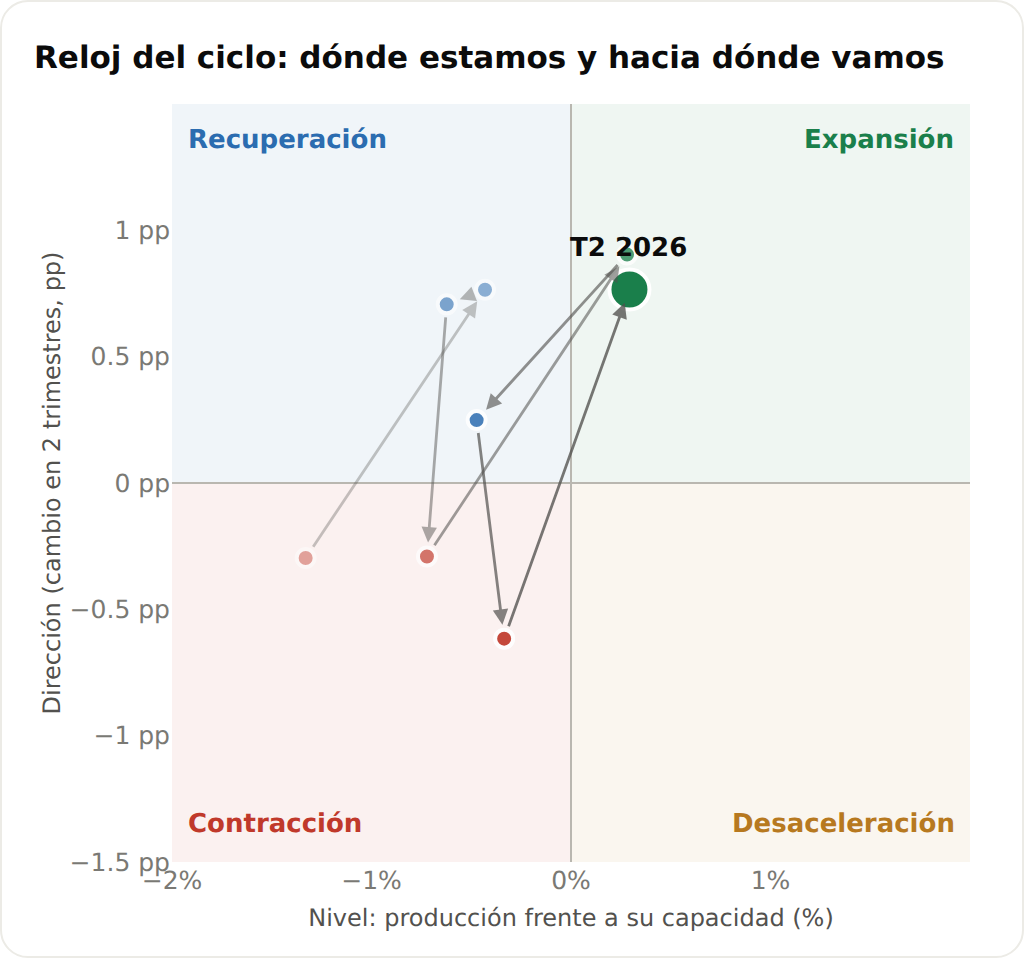
\includegraphics[width=0.48\linewidth]{fig_ciclo-reloj.png}
\vfill
{\sffamily\small Sitio: \url{https://stv-quant.github.io/ColombiaMacro-USBCali/} · Complementos: \textit{ColombiaMacro\_Beamer.pdf} y \textit{Manual\_ColombiaMacro.pdf}.}
\end{titlepage}

\tableofcontents
\newpage

% ================================================================
\needspace{14\baselineskip}
\section{Estructura de la exposición}

Formato: 20 minutos de exposición, 3 de demostración y 15 de preguntas. La secuencia sigue la de un
informe de política monetaria (actividad $\rightarrow$ precios $\rightarrow$ política $\rightarrow$ activos) y
termina en la lectura para el inversionista.

\begin{center}\small
\begin{tabularx}{\linewidth}{@{}rXr@{}}
\toprule
\textbf{Bloque} & \textbf{Contenido y mensaje} & \textbf{Min.}\\\midrule
1 & Pregunta y respuesta en una frase (portada de esta guía). & 1\\
2 & Obtención de datos: fuentes oficiales, descarga automática, controles (sección~\ref{sec:datos}). & 3\\
3 & Del dato al gráfico: transformación, convenciones, publicación (sección~\ref{sec:construccion}). & 3\\
4 & Actividad y mercado laboral: reloj, capacidad, sectores, empleo, informalidad (sección~\ref{sec:actividad}). & 4\\
5 & Precios, expectativas y política: inflación, implícitas, 5y5y, tasa real, curva TES (sección~\ref{sec:precios}). & 4\\
6 & Mercados y sector externo: dólar, ITCR, COLCAP por dentro, cuenta corriente, deuda (sección~\ref{sec:mercados}). & 2\\
7 & Lectura para el inversionista y señales a vigilar (sección~\ref{sec:inversion}). & 2\\
8 & Limitaciones y cierre (sección~\ref{sec:limites}). & 1\\
\midrule
 & Demostración en vivo (sección~\ref{sec:demo}). & 3\\
\bottomrule
\end{tabularx}
\end{center}

Regla para cada gráfico durante la exposición: \textbf{dato $\rightarrow$ cómo se construyó $\rightarrow$
qué dice hoy $\rightarrow$ qué implica}. Máximo 40 segundos por gráfico.

% ================================================================
\needspace{14\baselineskip}
\section{Obtención de los datos}
\label{sec:datos}

\needspace{8\baselineskip}
\subsection{Principios}
\begin{enumerate}
\item \textbf{Solo fuentes oficiales} (DANE, Banco de la República, Superfinanciera, MinHacienda vía BanRep, BVC).
Las dos excepciones de mercado (canasta del COLCAP y precios por acción) están declaradas.
\item \textbf{Sin intervención manual}: cada serie se descarga por programa, con su identidad verificada
(número de serie \emph{y} nombre). Si la fuente cambia la variable, el proceso falla en lugar de publicar otra.
\item \textbf{Trazabilidad}: cada actualización queda como un \emph{commit} en el repositorio con fecha y hora;
cualquier cifra se puede rastrear hasta su descarga.
\end{enumerate}

\needspace{8\baselineskip}
\subsection{Arquitectura}
\begin{center}
\begin{tikzpicture}[b/.style={draw=cmrule,fill=cmsoft,rounded corners=2pt,align=center,font=\sffamily\scriptsize,text width=22mm,minimum height=15mm},
  a/.style={-{Stealth[length=2mm]},color=cmmuted,thick}]
\node[b] (f) {\textbf{Fuentes}\\API BanRep\\Anexos DANE\\iShares, Yahoo};
\node[b,right=4mm of f] (d) {\textbf{Descarga}\\\texttt{fuentes/*.py}\\identidad + rangos};
\node[b,right=4mm of d] (c) {\textbf{Datos}\\CSV versionados\\en \texttt{data/}};
\node[b,right=4mm of c] (m) {\textbf{Modelo}\\fórmulas y\\veredicto};
\node[b,right=4mm of m] (s) {\textbf{Sitio}\\HTML estático\\+ Plotly};
\draw[a] (f)--(d); \draw[a] (d)--(c); \draw[a] (c)--(m); \draw[a] (m)--(s);
\node[font=\sffamily\scriptsize,color=cmmuted,below=2mm of c] {GitHub Actions: cada hora en días hábiles + corrida completa nocturna};
\end{tikzpicture}
\end{center}

\needspace{8\baselineskip}
\subsection{Fuentes y método de descarga}
\begin{center}\small
\begin{tabularx}{\linewidth}{@{}p{0.27\linewidth}p{0.2\linewidth}Xp{0.1\linewidth}@{}}
\toprule
\textbf{Variable} & \textbf{Fuente} & \textbf{Método} & \textbf{Frec.}\\\midrule
PIB real (orig. y desest.), PIB nominal, 12 sectores & DANE & Anexos \texttt{anex-Produccion*} (Cuadros 1 y 4); se localiza el enlace vigente en la página técnica y se valida estructura y trimestre & Trim.\\
ISE & DANE & Anexo \texttt{anex-ISE-9actividades} & Mens.\\
Desempleo, ocupación, participación & DANE, GEIH & Anexo desestacionalizado & Mens.\\
Informalidad (nacional, 23 ciudades, 13 ramas) & DANE, GEIH & Anexo \texttt{anex-GEIHEISS} (hojas de proporción y ramas) & Mens.\\
IPC, inflación básica, meta & DANE / BanRep & API estadística BanRep (series 15000, 15390, 853) & Mens.\\
Tasa de política & BanRep & Serie 59 + registro del anuncio de la Junta & Diaria\\
Curvas cero cupón TES pesos y UVR (1, 5, 10 años) & BanRep & Series 15272–15277 & Diaria\\
TRM & Superfinanciera vía BanRep & Serie 1 & Diaria\\
COLCAP & BVC vía BanRep & Serie oficial del índice & Diaria\\
Canasta y pesos del COLCAP & iShares MSCI COLCAP & Archivo diario de tenencias del fondo & Diaria\\
Precios por acción & Yahoo Finance & Cierres semanales \texttt{TICKER.CL} & Semanal\\
ITCR, cuenta corriente, IED, reservas & BanRep & Series 235, 15290, 15133, 15051 & Mens./Trim.\\
Deuda bruta GNC & MinHacienda vía BanRep & Serie 15328 & Anual\\
\bottomrule
\end{tabularx}
\end{center}

\textbf{Decisiones de la Junta.} La serie oficial registra la nueva tasa el día en que \emph{rige}, no el día del
anuncio. Para no mostrar un dato viejo el día de la decisión, el anuncio se registra en
\archivo{data/decisiones\_banrep.csv} y el tablero lo muestra como “anunciada” hasta que entra a la serie
(caso actual: 30-sep-2026, 12,00\% $\rightarrow$ 12,25\%, rige el 1-oct).

\needspace{8\baselineskip}
\subsection{Calendario de actualización}
\begin{itemize}
\item \textbf{Cada hora, lunes a viernes, 7:07–18:07 (hora de Colombia)}: series diarias (tasa de política, TES,
TRM, COLCAP). Se publica solo si llegó un dato nuevo.
\item \textbf{Todos los días, 19:30}: corrida completa (DANE, BanRep, canasta y precios de acciones).
\item Una fuente que falla conserva su último dato válido y queda registrada en el estado de fuentes; no detiene
la publicación.
\end{itemize}

\needspace{8\baselineskip}
\subsection{Controles de calidad}
\begin{center}\small
\begin{tabularx}{\linewidth}{@{}p{0.28\linewidth}X@{}}
\toprule
\textbf{Control} & \textbf{Regla}\\\midrule
Identidad & Número de serie y nombre deben coincidir con el catálogo.\\
Fechas & Sin duplicados, sin fechas futuras, sin meses o trimestres faltantes; el último trimestre del anexo
debe coincidir con su nombre de archivo.\\
Rangos & Límites plausibles por serie (p.\,ej. crecimiento anual del PIB $|x|<40\%$).\\
Saltos aislados & Valor que se aleja $>2$\,pp de ambos vecinos que difieren $<1$\,pp: se conserva en el CSV,
se lista en \archivo{alertas\_datos.csv} y se excluye de los cálculos.\\
Identidades contables & $TD = 1 - TO/TGP$; inflación mensual compuesta a 12 meses = anual ($\pm0{,}04$\,pp);
la suma de informales por rama reproduce la tasa nacional.\\
Pruebas & 63 pruebas automáticas corren antes y después de cada descarga.\\
\bottomrule
\end{tabularx}
\end{center}

% ================================================================
\needspace{14\baselineskip}
\section{Construcción de los gráficos}
\label{sec:construccion}

\needspace{8\baselineskip}
\subsection{Proceso común}
\begin{enumerate}
\item \textbf{Carga}: los CSV de \archivo{data/} se leen en un objeto único (\texttt{modelo.cargar}).
\item \textbf{Transformación}: las fórmulas (variaciones, filtro HP, Fisher, forwards, índices) están en
\texttt{analitica.py} y \texttt{modelo.py} y se recalculan en cada corrida; nada se guarda precalculado.
\item \textbf{Figura}: cada gráfico se arma en Python con Plotly (\texttt{sitio/construir.py}): panel principal +
panel inferior de cambio + franja de cifras clave + pie con fuente y metodología.
\item \textbf{Publicación}: la figura se serializa en JSON dentro de un HTML estático (español e inglés). En el
navegador, \texttt{app.js} la dibuja y aplica el horizonte elegido (3, 5, 10 años o todo), recalculando los
ejes con los datos visibles.
\item \textbf{Descarga}: cada tabla usada se ofrece en CSV para replicar el cálculo.
\end{enumerate}

\needspace{8\baselineskip}
\subsection{Convenciones}
\begin{itemize}
\item \textbf{Un eje, una unidad} por panel. La única excepción es el PIB en dólares (eje derecho, marcado como referencia).
\item \textbf{Panel de cambio}: debajo de cada serie, su variación frente a hace un año (tasas en puntos
porcentuales, niveles en \%); el PIB y la brecha, frente al trimestre anterior.
\item \textbf{Franja de cifras}: último dato, fecha y variación, con flecha y color según el signo.
\item \textbf{Referencias normativas} dibujadas en el gráfico: meta 3\% $\pm$1\,pp, tasa neutral 2,7–3,0\%,
capacidad de la economía.
\item \textbf{Unidades}: pesos colombianos (COP); “billón” = $10^{12}$. Fechas al cierre del periodo.
\item \textbf{Pie de cada gráfico}: fuente; el signo “?” despliega la metodología exacta.
\end{itemize}

% ================================================================
\clearpage
\needspace{14\baselineskip}
\section{Actividad y mercado laboral}
\label{sec:actividad}

\needspace{8\baselineskip}
\subsection{Reloj del ciclo}
\grafico{fig_ciclo-reloj.png}{0.55}
{Brecha del producto $g_t = 100(\ln Y_t - \ln Y^*_t)$ con $Y$ el PIB real desestacionalizado y $Y^*$ la
tendencia de un filtro Hodrick-Prescott \emph{en tiempo real} ($\lambda=1600$; cada trimestre usa solo datos
disponibles a esa fecha; 2020T2–2021T2 interpolados solo para estimar la tendencia). Eje vertical:
$\Delta_2 g_t = g_t - g_{t-2}$. Fase = cuadrante (metodología OCDE).}
{Derecha: produce por encima de su capacidad. Arriba: la distancia aumenta. El ciclo gira en sentido horario:
expansión $\rightarrow$ desaceleración $\rightarrow$ contracción $\rightarrow$ recuperación. Hoy: T2 2026 en
expansión ($g=+0{,}3\%$, $\Delta_2 g=+0{,}77$\,pp), tras dos años alrededor de cero.}
{La fase resume el entorno para todos los activos (sección~\ref{sec:inversion}). Una brecha positiva y creciente
anticipa presión inflacionaria y tasas altas por más tiempo. Cerca del origen la fase es frágil: un trimestre
basta para cambiar de cuadrante.}

\needspace{8\baselineskip}
\subsection{Producción frente a su capacidad}
\grafico{fig_capacidad.png}{0.6}
{Capacidad $Y^*_t = Y_t\,e^{-g_t/100}$, en billones de COP de 2015 por trimestre. Área verde: producción
sobre la capacidad; naranja: holgura. Contrastes: HP de dos colas y Hamilton (2018); hoy los tres métodos dan
brecha positiva (rango +0,3\% a +2,3\%).}
{Es la frontera de posibilidades de producción en el tiempo: la línea punteada es lo máximo sostenible sin
generar inflación. 2020 muestra la caída de $\approx$18\% bajo la capacidad; 2022 el sobrecalentamiento; desde
2023 holgura leve; hoy, levemente por encima.}
{Holgura $\Rightarrow$ espacio para bajar tasas. Sobrecalentamiento $\Rightarrow$ alzas y presión sobre bonos
largos. El crecimiento potencial estimado ($\approx$2,4\% anual) es la referencia para juzgar si un dato de PIB
es “alto”.}

\needspace{8\baselineskip}
\subsection{Crecimiento del PIB y del ISE}
\grafico{fig_crec.png}{0.6}
{Barras: $100(Y_t/Y_{t-4}-1)$ con PIB real original. Línea: ISE desestacionalizado, variación anual.
Punteada: crecimiento de la tendencia HP. Panel inferior: cambio frente al trimestre anterior.}
{T2 2026: +3,5\% anual, sobre el potencial (2,4\%). El ISE de julio (+1,1\% anual; +5,8\% anualizado en 3
meses) es el primer dato del T3.}
{El ISE adelanta el PIB dos meses: es el dato a seguir entre publicaciones trimestrales.}

\needspace{8\baselineskip}
\subsection{Crecimiento real por año}
\grafico{fig_pib-anual.png}{0.6}
{Barras: $100(\sum_q Y_{a,q}/\sum_q Y_{a-1,q}-1)$ con el PIB real original de los cuatro trimestres de cada año; barra
clara: últimos 12 meses frente a los 12 previos. Punteada verde: ritmo habitual (tendencia HP); discontinua: promedio
2010–2019.}
{Últimos 12 meses al T2 2026: +2,9\% real; 2025: +2,6\%; promedio 2010–2019: 3,7\%. Desde 2023 la economía crece por
debajo de su promedio histórico, aunque el último trimestre (3,5\%) muestra aceleración.}
{La versión anual filtra el ruido trimestral: es la referencia para comparar con proyecciones de crecimiento y con el
potencial. Crecer por debajo del promedio histórico implica menor expansión de ventas y de recaudo.}

\needspace{8\baselineskip}
\subsection{Crecimiento por sector}
\grafico{fig_sec-barras.png}{0.6}
{12 agrupaciones CIIU Rev.\,4 (volúmenes encadenados, datos originales). Crecimiento anual; raya negra = un año
antes. Aporte $c_{i,t}=(Y_{i,t}-Y_{i,t-4})/VA_{t-4}$. El selector y el clic en el mapa permiten ver cualquier
trimestre desde 2009.}
{T2 2026: lidera Gobierno, educación y salud (+10,0\%, aporte 1,8\,pp de los 3,5\% del PIB). Caen agro
(--2,1\%) e información y comunicaciones (--0,1\%). Industria y construcción, alrededor de 2\%.}
{Crecimiento concentrado en gasto público: menor calidad y sostenibilidad (depende de la caja fiscal). Los
sectores cíclicos privados (industria, construcción, comercio) crecen por debajo del total.}

\grafico{fig_sec-mapa.png}{0.6}
{Mapa de calor del crecimiento anual por sector y trimestre; escala recortada en $\pm12\%$ para que 2020 no oculte
el resto; sectores ordenados por peso.}
{Muestra de un vistazo la amplitud del ciclo: columnas azules completas = expansión generalizada; columnas mixtas
= crecimiento concentrado.}
{Permite identificar sectores con impulso persistente (varios trimestres azules) frente a rebotes de un trimestre.}

\needspace{8\baselineskip}
\subsection{Desempleo}
\grafico{fig_desempleo.png}{0.6}
{Tasa de desempleo desestacionalizada (DANE, GEIH); promedio móvil de 3 meses. Panel: cambio frente a un año antes.}
{Julio 2026: 8,3\% (9,0\% un año antes): mercado laboral más estrecho, coherente con la brecha positiva.}
{Desempleo a la baja sostiene el consumo y los salarios, pero alimenta la inflación de servicios: argumento a
favor de una política restrictiva prolongada.}

\needspace{8\baselineskip}
\subsection{Informalidad}
\grafico{fig_informal.png}{0.6}
{Proporción de ocupados informales (definición DANE 2023, alineada con la OIT), trimestres móviles desde 2021:
nacional, 13 y 23 ciudades.}
{Julio 2026: 54,6\% nacional, 40,6\% en las 13 ciudades. La brecha entre ambas refleja el peso del empleo rural y
por cuenta propia.}
{Alta informalidad reduce la base tributaria y la transmisión de la política monetaria (menos crédito formal):
limita el efecto de las tasas sobre la demanda.}

\grafico{fig_inf-ramas.png}{0.6}
{Informales / ocupados por rama, total nacional; raya = un año antes.}
{Mayor informalidad: agro (85\%), alojamiento y comida (73\%), construcción y transporte (69\%). Menor: finanzas (12\%) y gobierno, educación y salud (12\%).}
{Sectores con alta informalidad tienen menor productividad y acceso a crédito; su crecimiento se traduce menos en recaudo.}

\graficoancho{fig_inf-ciudades.png}{0.8}
{Informalidad en las 23 ciudades y áreas metropolitanas; en azul las 13 principales (Bogotá, Medellín A.M., Cali A.M.,
Barranquilla A.M., Bucaramanga A.M., Manizales A.M., Pasto, Pereira A.M., Cúcuta A.M., Ibagué, Montería, Cartagena,
Villavicencio).}
{Dispersión amplia: de 33\% en Bogotá a 65\% en Sincelejo. Por encima de 60\%: Sincelejo, Riohacha, Cúcuta, Montería y
Valledupar; por debajo de 40\%: Bogotá, Manizales, Tunja y Medellín.}
{Útil para decisiones regionales (consumo formal, crédito, inmobiliario): la formalidad local aproxima el mercado
bancarizable.}

% ================================================================
\needspace{14\baselineskip}
\section{Precios, expectativas y política monetaria}
\label{sec:precios}

\needspace{8\baselineskip}
\subsection{Inflación}
\grafico{fig_inf.png}{0.6}
{Inflación anual $100(IPC_t/IPC_{t-12}-1)$ (último dato = cifra publicada por el DANE); inflación sin alimentos ni
regulados (BanRep). Franja: meta 3\% $\pm$1\,pp.}
{Agosto 2026: 6,24\% (5,1\% un año antes), básica 6,12\%; acelera 0,4\,pp en 3 meses. Fuera del rango meta y
con la básica casi igual a la total: presión generalizada, no solo choques de alimentos.}
{Inflación alta y acelerando $\Rightarrow$ tasas nominales altas; los activos indexados (TES UVR) protegen frente a sorpresas.}

\needspace{8\baselineskip}
\subsection{Inflación que descuenta el mercado}
\grafico{fig_espera.png}{0.6}
{Inflación implícita (\emph{breakeven}) por plazo $h$: $\pi^{BE}_h = 100\left[\frac{1+i^{COP}_h}{1+r^{UVR}_h}-1\right]$ con
las curvas cero cupón de los TES (Fisher exacto).}
{Hoy: 7,1\% a 1 año, 6,0\% a 5 y a 10 años. Contiene primas por riesgo inflacionario y liquidez: se lee como cota
superior de la expectativa pura. Validación: antes de 2020 pronosticó mejor que la caminata aleatoria (RMSE 1,70
vs 2,08\,pp).}
{Si se espera una inflación mayor que el \emph{breakeven}, el TES UVR rinde más que el TES en pesos; si menor, al revés.}

\needspace{8\baselineskip}
\subsection{Trayectoria esperada a 10 años}
\graficoancho{fig_tray.png}{0.95}
{Tramos que encadenan el \emph{breakeven} a 10 años: año 1 $=b_1$; años 1–5 $=[(1+b_5)^5/(1+b_1)]^{1/4}-1$;
años 5–10 $=[(1+b_{10})^{10}/(1+b_5)^5]^{1/5}-1$ (la 5y5y). Se dibujan hacia el futuro junto a la lectura de hace un año.}
{El mercado descuenta 7,1\% el próximo año, 5,8\% entre el año 1 y el 5 y 6,0\% entre el 5 y el 10. Ningún tramo
regresa al rango meta y todos están por encima de lo esperado hace un año.}
{Pérdida de credibilidad de la meta $\Rightarrow$ prima de riesgo inflacionario en los bonos largos en pesos.
Un descenso de los tramos hacia la franja verde sería la señal de reanclaje.}

\needspace{8\baselineskip}
\subsection{Anclaje de las expectativas (5y5y)}
\graficoancho{fig_anclaje.png}{0.8}
{Forward 5y5y: $[(1+b_{10})^{10}/(1+b_5)^5]^{1/5}-1$, promedio semanal. Regla: desanclada si supera 4\% (techo del rango meta).}
{6,0\%: desanclada. No es un pronóstico de su propia serie: cada punto es lo que el mercado esperaba ese día para
la inflación promedio entre 5 y 10 años adelante.}
{Es el termómetro de credibilidad del banco central y el principal determinante de la prima a plazo de los TES largos.}

\needspace{8\baselineskip}
\subsection{Tasa de política e inflación}
\graficoancho{fig_politica.png}{0.8}
{Tasa de intervención (escalones en cada decisión de la Junta) frente a la inflación anual. La estrella marca la
decisión anunciada que aún no rige.}
{12,00\% $\rightarrow$ 12,25\% (anuncio 30-sep-2026, rige 1-oct). Hace un año: 9,25\%. Ciclo de alzas en curso.}
{La dirección de la tasa domina el retorno de los bonos cortos y el costo de financiación de las empresas.}

\needspace{8\baselineskip}
\subsection{Tasa real ex ante}
\graficoancho{fig_real.png}{0.8}
{$r^{ea} = 100\,[(1+TPM)/(1+\pi^{BE}_1)-1]$: tasa del Banco descontada la inflación \emph{esperada}
(“ex ante” = antes de que ocurra). Franja gris: neutral 2,7–3,0\% (equipo técnico de BanRep). Postura: restrictiva
si $r^{ea}>3{,}5\%$, expansiva si $<2{,}2\%$.}
{Con la nueva tasa: $1{,}1225/1{,}0708-1\approx4{,}8\%$, por encima de la neutral: política restrictiva.}
{Tasa real alta = rendimiento real atractivo en renta fija corta y freno al crédito y a la valoración de acciones.}

\needspace{8\baselineskip}
\subsection{Curva de los TES}
\grafico{fig_curva-tes.png}{0.6}
{Tasas cero cupón a 1, 5 y 10 años del día elegido (BanRep); líneas finas: cierres de año. Pendiente = 10a $-$ 1a.}
{Hoy 12,42\% / 12,90\% / 13,06\%: curva casi plana (pendiente 0,64\,pp). El TES a 10 años supera la tasa de política
en 1,06\,pp.}
{Una curva plana con tasa alta indica que el mercado no descuenta recortes pronto. Rendimiento real a 10
años (TES UVR cero cupón): 6,6\%.}

\grafico{fig_curva-hist.png}{0.6}
{Serie diaria de las tasas cero cupón a 1, 5 y 10 años desde 2003.}
{Ubica el nivel actual frente a la historia: el TES a 10 años (13,1\%) solo fue superado en 2022–2023 (máximo 15,4\% en octubre de 2022).}
{Inversión de la curva (1a > 10a) ha precedido desaceleraciones; su normalización suele acompañar el inicio de recortes.}

% ================================================================
\needspace{14\baselineskip}
\section{Mercados y sector externo}
\label{sec:mercados}

\needspace{8\baselineskip}
\subsection{Dólar (TRM) y tasa de cambio real}
\grafico{fig_dolar.png}{0.6}
{TRM (pesos por dólar), promedio semanal; panel: variación anual.}
{3.341 pesos por dólar: el peso se apreció 14,4\% en 12 meses.}
{Para el inversionista extranjero el tipo de cambio domina el retorno: el COLCAP subió 36\% en pesos y 65\% en dólares.}

\graficoancho{fig_itcr.png}{0.8}
{ITCR-IPC (2010 = 100): tipo de cambio ajustado por la inflación de Colombia frente a la de sus socios comerciales.}
{95,7 (agosto): el peso está más caro en términos reales que en el año base. Valores bajos restan competitividad a
las exportaciones no minero-energéticas.}
{Un peso real fuerte reduce el margen de seguridad para nuevas entradas en pesos: el riesgo de reversión cambiaria es mayor.}

\needspace{8\baselineskip}
\subsection{COLCAP}
\grafico{fig_bolsa.png}{0.6}
{Índice COLCAP oficial (BVC vía BanRep), índice de precios sin dividendos, cierre semanal; en dólares = puntos / TRM.}
{2.559 puntos (29-sep), +36,5\% en 12 meses en pesos, $-$2,6\% desde su máximo.}
{Rentabilidad sin dividendos; el retorno total es mayor. Ver la composición antes de concluir que “la bolsa” sube.}

\needspace{8\baselineskip}
\subsection{La bolsa por dentro: equiponderado y 7 Magníficas}
\grafico{fig_indices.png}{0.6}
{Canasta y pesos: tenencias diarias del fondo iShares MSCI COLCAP (agrupadas por emisor). Precios: cierres semanales.
Equiponderado: $I_t=I_{t-1}(1+\bar r_t)$, promedio simple de retornos semanales; 7 Magníficas: igual, con las 7
empresas de mayor peso. Base 100 al inicio del horizonte. Usa la canasta actual hacia atrás (sesgo de supervivencia).}
{12 meses: COLCAP +38,1\%, 7 Magníficas +35,2\%, equiponderado +28,8\%. COLCAP > equiponderado: el alza se concentra
en las empresas grandes; no es generalizada.}
{Comprar el índice es, en la práctica, comprar las grandes. La amplitud (equiponderado) confirma o niega la solidez del alza.}

\grafico{fig_pesos.png}{0.6}
{Peso de cada emisor en el fondo que replica el COLCAP (sin efectivo).}
{Las 7 Magníficas suman 85,1\%: Grupo Cibest 37,8\%, Grupo Sura 12,0\%, Ecopetrol 8,9\%, ISA 8,8\%, Grupo Argos
7,8\%, GEB 5,3\%, Cementos Argos 4,4\%.}
{Riesgo de concentración: el índice es mayoritariamente financiero; su sensibilidad a tasas y crédito es mayor que la de una canasta diversificada.}

\needspace{8\baselineskip}
\subsection{Cuenta corriente y deuda pública}
\grafico{fig_cc.png}{0.6}
{Saldo de la cuenta corriente (\% del PIB), balanza de pagos BanRep.}
{T2 2026: $-$3,5\% del PIB: el país necesita financiación externa equivalente.}
{Déficit externo + peso fuerte = dependencia de flujos de capital; un cambio en el apetito global por riesgo se transmite al peso y a los TES.}

\grafico{fig_deuda.png}{0.6}
{Deuda bruta del Gobierno Nacional Central (\% del PIB), cierre anual (MinHacienda vía BanRep).}
{62,9\% del PIB en 2025, en la parte alta de su historia.}
{La deuda alta sostiene la prima de riesgo soberano y limita el espacio fiscal; junto con el crecimiento liderado por
gasto público, es el principal riesgo para los TES largos.}

% ================================================================
\needspace{14\baselineskip}
\section{Lectura para el inversionista}
\label{sec:inversion}

\begin{alerta}[Alcance]
El tablero describe el estado de la economía con datos oficiales; no es una recomendación de inversión ni un
pronóstico. Las relaciones siguientes son regularidades históricas, no reglas.
\end{alerta}

\needspace{8\baselineskip}
\subsection{Fase del ciclo y comportamiento típico de los activos}
\begin{center}\small
\begin{tabularx}{\linewidth}{@{}p{0.15\linewidth}XXX@{}}
\toprule
\textbf{Fase} & \textbf{Tasas y curva} & \textbf{Renta fija} & \textbf{Acciones y peso}\\\midrule
Expansión & Tasas al alza; curva se aplana & Bonos largos bajo presión & Cíclicas y financieras favorecidas\\
Desaceleración & Tasa cerca del máximo & Duración empieza a ganar & Defensivas (servicios públicos) relativamente mejor\\
Contracción & Recortes; curva se empina & Bonos largos ganan & Acciones caen; peso tiende a depreciarse\\
Recuperación & Tasas bajas, curva empinada & Ganancias de los recortes ya realizadas & Cíclicas lideran el rebote\\
\bottomrule
\end{tabularx}
\end{center}

\needspace{8\baselineskip}
\subsection{Lectura actual (30 de septiembre de 2026)}
\begin{center}\small
\begin{tabularx}{\linewidth}{@{}p{0.22\linewidth}p{0.25\linewidth}X@{}}
\toprule
\textbf{Dimensión} & \textbf{Dato} & \textbf{Implicación}\\\midrule
Ciclo & Expansión; brecha +0,3\% (3/3 métodos) & Crecimiento sobre el potencial, pero cerca del origen: fase frágil.\\
Composición & Gobierno aporta 1,8 de 3,5\,pp & Crecimiento dependiente de gasto público.\\
Inflación & 6,24\% y acelerando & Fuera de la meta; presión generalizada (básica 6,12\%).\\
Expectativas & 5y5y 6,0\% & Desancladas: prima inflacionaria en bonos largos.\\
Política & 12,25\%; real ex ante $\approx$4,8\% & Restrictiva y en ciclo de alzas.\\
Curva TES & 12,4 / 12,9 / 13,1\%; pendiente 0,64\,pp & Mercado no descuenta recortes cercanos; rendimiento real alto.\\
Peso & 3.341; $-$14,4\% en 12 meses; ITCR 95,7 & Peso fuerte en términos reales: riesgo de reversión.\\
Bolsa & COLCAP +38\%; equiponderado +29\% & Alza concentrada en emisores grandes (85\% en 7 empresas).\\
Externo y fiscal & CC $-$3,5\% PIB; deuda 62,9\% PIB & Dependencia de flujos externos y prima soberana.\\
\bottomrule
\end{tabularx}
\end{center}

\textbf{Síntesis.} Economía en expansión con inflación desanclada y política restrictiva: el entorno favorece
rendimientos reales altos en renta fija y exige cautela con la duración mientras las expectativas no bajen. El
retorno en dólares de los activos colombianos depende críticamente de un peso que ya se apreció. La bolsa sube,
pero concentrada en pocos emisores.

\needspace{8\baselineskip}
\subsection{Señales a vigilar}
\begin{center}\small
\begin{tabularx}{\linewidth}{@{}p{0.3\linewidth}p{0.2\linewidth}X@{}}
\toprule
\textbf{Indicador} & \textbf{Umbral} & \textbf{Qué cambiaría}\\\midrule
Brecha (reloj) & $\Delta_2 g<0$ & Paso a desaceleración: fin probable del ciclo de alzas.\\
Inflación anual y básica & 3 meses cediendo & Espacio para recortes; favorece duración.\\
5y5y & $<4\%$ & Reanclaje: compresión de la prima en TES largos.\\
Tasa real ex ante & $<3{,}5\%$ & Fin de la postura restrictiva.\\
Pendiente 10a $-$ 1a & $<0$ & Curva invertida: señal de desaceleración.\\
COLCAP vs. equiponderado & equiponderado > COLCAP & Alza más amplia y sólida.\\
TRM y cuenta corriente & depreciación $>10\%$ anual & Salida de capitales; presión inflacionaria importada.\\
\bottomrule
\end{tabularx}
\end{center}

% ================================================================
\needspace{14\baselineskip}
\section{Limitaciones}
\label{sec:limites}
\begin{enumerate}
\item \textbf{Vintage única}: la historia corresponde a la última publicación del DANE; el HP en tiempo real elimina
la información futura del filtro, no las revisiones.
\item \textbf{La fase depende del método}: coincidencia de fase HP en tiempo real vs. Hamilton, 43\%; de signo, 65–78\%.
Por eso se muestra el rango entre métodos.
\item \textbf{Implícitas con primas} (riesgo inflacionario, liquidez del TES UVR, rezago de indexación): cota superior de la expectativa.
\item \textbf{Neutral externa}: estimación de BanRep con incertidumbre; la conclusión (restrictiva) se mantiene en todo su rango.
\item \textbf{COLCAP sin dividendos}; índices equiponderado y 7 Magníficas con canasta actual hacia atrás (sesgo de supervivencia).
\item \textbf{Informalidad desde 2021}: cambio de definición del DANE; no se empalma con la serie anterior.
\end{enumerate}

% ================================================================
\needspace{14\baselineskip}
\section{Preguntas técnicas previsibles}
\begin{description}[style=nextline,leftmargin=0pt]
\item[¿Por qué el filtro HP si Hamilton (2018) lo critica?]
Se usa en tiempo real (sin información futura) y se contrasta con HP de dos colas y Hamilton; el tablero muestra
el rango. Hoy los tres coinciden en el signo.
\item[¿Por qué $\lambda=1600$ y por qué interpolar 2020–2021?]
1600 es el estándar trimestral. La interpolación solo afecta la estimación de la tendencia; la brecha se mide contra
el dato observado. Sin ella, una caída de 17,6\% en un trimestre deforma la tendencia de 2019 a 2023.
\item[¿La 5y5y es un pronóstico?]
Es lo que descuentan los bonos para la inflación promedio entre los años 5 y 10, incluidas primas. No es pronóstico
del tablero ni del Banco.
\item[¿Por qué la tasa anunciada aparece antes que en la serie oficial?]
La serie registra la tasa cuando rige; el anuncio se registra aparte y se marca como “anunciada”.
\item[¿Por qué los aportes sectoriales no suman el PIB?]
Los volúmenes encadenados no son aditivos y los aportes suman al valor agregado, no al PIB (que incluye impuestos netos).
\item[¿Por qué pesos de iShares y no de la BVC?]
El fondo replica el índice y publica su composición diaria en un archivo estable; la BVC no ofrece una fuente
automatizable equivalente. La diferencia es de décimas.
\item[¿Se puede verificar una cifra?]
Sí: cada gráfico cita su fuente y método, cada tabla se descarga en CSV y cada actualización es un \emph{commit} con fecha.
\end{description}

% ================================================================
\needspace{14\baselineskip}
\section{Demostración en vivo}
\label{sec:demo}
\begin{enumerate}
\item Portada: resumen automático y tarjetas (fecha de los datos y hora de construcción).
\item Reloj del ciclo: mover el selector de trimestre y mostrar el recorrido 2020–2026.
\item Horizonte “Todo” en la barra superior: 2020 completo en los gráficos.
\item Sectores: clic en una columna del mapa $\rightarrow$ las barras muestran ese trimestre.
\item Curva TES: clic en la historia para fijar una fecha y comparar con hoy.
\item Signo “?” al pie de un gráfico: metodología; descargar un CSV.
\end{enumerate}
\textbf{Respaldo}: capturas de esta guía y el PDF de diapositivas, por si falla la conexión. Abrir el sitio una vez antes
de la sesión (Ctrl+F5) para cargar la última versión.

\end{document}
